\begin{frame}
    \centering
    \begin{figure}[H]
        
\includegraphics[keepaspectratio, width=0.7\paperwidth, height=\paperheight]{Logos/LeeLogo}
    \end{figure}
    Statistik: Daten beschreiben und Schlüsse ziehen\\
    \emoji{chart-increasing} Kapitel 1: \textbf{Von beschreibend zu schliessend}
\end{frame}

\fboxsep=.6pt

\begin{frame}{Wozu Statistik?}
    \begin{itemize}[<+->]
        \item Statistik hilft uns, aus Daten sinnvolle Aussagen zu gewinnen
        \item Schützt vor Täuschung durch Einzelfälle, Ausreisser und geschickte Grafiken
        \item Das Zusammenspiel:
              \begin{center}
                  \textbf{Fragestellung\ $\rightarrow$\ Daten\ $\rightarrow$\ Beschreibung\ $\rightarrow$\ Schlussfolgerung}
              \end{center}
    \end{itemize}

    \vspace{1em}
    \begin{block}{Wichtig}
        Statistik ist keine Rechenakrobatik, sondern vor allem \textbf{sauberes Denken}:\\
        Welche Daten liegen vor? Was darf man damit berechnen? Was bedeutet das Ergebnis?
    \end{block}
\end{frame}

\begin{frame}{Ablauf im Modul}
    \begin{enumerate}[<+->]
        \item \textbf{Gute Fragestellungen}: Variabilität, Zielgruppe, Vergleich
        \item \textbf{Daten beschreiben}: Skalenniveaus, Kennzahlen, Diagramme
        \item \textbf{Schliessende Statistik}: Unterschiede mit Unsicherheit beurteilen
        \item \textbf{Eigene Fragestellung}: Erarbeitetes auf eigenes Thema anwenden
    \end{enumerate}

    \vspace{0.8em}
    \begin{block}{Ziel}
        Mehr Transfer: möglichst mit Fragestellungen der SuS arbeiten.
    \end{block}
\end{frame}

\begin{frame}{Was ist eine gute statistische Fragestellung?}
    \begin{itemize}[<+->]
        \item Eine statistische Frage braucht eine \textbf{variable Grösse}
        \item \textbf{Nicht ideal}: \enquote{Wer ist der Grösste in der Klasse?}
        \item \textbf{Besser}: \enquote{Wie ist die Verteilung der Körpergrössen in der Klasse?}
        \item Die Frage soll Zielgruppe und Vergleich klar machen
    \end{itemize}
\end{frame}

\begin{frame}{Repräsentativ und signifikant}
    \begin{itemize}[<+->]
        \item \textbf{Repräsentativ}: Stichprobe passt zur Grundgesamtheit
        \item Beispiel: Nur Lee-Lernende (15--17) \Rightarrow Aussage zuerst nur für diese Gruppe
        \item \textbf{Signifikant}: beobachteter Effekt unter Zufallsmodell eher unwahrscheinlich
        \item Signifikant heisst nicht automatisch \enquote{gross} oder \enquote{wichtig}
    \end{itemize}
\end{frame}

\begin{frame}{Skalenniveaus: Überblick}
    \begin{itemize}[<+->]
        \item Das \textbf{Skalenniveau} bestimmt, welche Rechnungen sinnvoll sind
        \item Zwei wichtige Fragen:
              \begin{enumerate}
                  \item Gibt es eine \textbf{Reihenfolge} (mehr/weniger)?
                  \item Sind \textbf{Abstände} oder \textbf{Verhältnisse} sinnvoll?
              \end{enumerate}
    \end{itemize}

    \vspace{1em}
    \only<4->{
        \begin{table}[H]
            \centering
            \tiny
            \begin{tabular}{l c c c l}
                \toprule
                \textbf{Niveau}    & \textbf{Ordnung} & \textbf{Abstände} & \textbf{Nullpunkt} & \textbf{Beispiele}                    \\
                \midrule
                Nominal            & \xmark           & \xmark            & \xmark             & Wohnort, Musikgenre                   \\
                Ordinal            & \cmark           & \xmark            & \xmark             & Schulnoten, Zufriedenheit (1--5)      \\
                Intervall          & \cmark           & \cmark            & \xmark             & Temperatur in $^{\circ}$C                      \\
                Verhältnis (Ratio) & \cmark           & \cmark            & \cmark             & Länge, Gewicht, Zeit, Temp. in Kelvin \\
                \bottomrule
            \end{tabular}
        \end{table}
    }
\end{frame}

\begin{frame}{Skalenniveaus: Statistische Verfahren}
    \begin{table}[H]
        \centering
        \scriptsize
        \begin{tabular}{l l l l}
            \toprule
            \textbf{Niveau} & \textbf{Zentrale Lage} & \textbf{Streuung} & \textbf{Visualisierung}      \\
            \midrule
            Nominal         & Modus                  & ---               & Balken-, Kreisdiagramm       \\
            Ordinal         & Median, Modus          & \gls{IQR}        & Boxplot, Balkendiagramm      \\
            Intervall       & Mittelwert, Median     & \gls{SD}, \gls{IQR} & Histogramm, Boxplot      \\
            Verhältnis      & Mittelwert, Median     & \gls{SD}, \gls{IQR} & Histogramm, Boxplot, Scatter \\
            \bottomrule
        \end{tabular}
    \end{table}

    \vspace{1em}
    \begin{block}{Merke}
        Je höher das Skalenniveau, desto mehr Rechenoperationen sind möglich.\\
        Bei Unsicherheit: Lieber ein niedrigeres Niveau wählen (konservativer Ansatz).
    \end{block}
\end{frame}

\begin{frame}{Übungen im Skript: Skalenniveaus}
    \begin{itemize}
        \item \aufgabebox{1.1: Skalenniveaus zuordnen}
    \end{itemize}
\end{frame}

\begin{frame}{Zentrale Lage: Mittelwert und Median}
    \begin{minipage}[c]{0.48\linewidth}
        \textbf{Mittelwert} (arithmetisches Mittel):
        \[
            \bar{x} = \frac{1}{n}\sum_{i=1}^{n} x_i
        \]
        \begin{itemize}
            \item Alle Werte werden berücksichtigt
            \item Reagiert stark auf Ausreisser
        \end{itemize}
    \end{minipage}\hfill
    \begin{minipage}[c]{0.48\linewidth}
        \textbf{Median}:
        \begin{itemize}
            \item Mittlerer Wert der sortierten Daten
            \item Bei gerader Anzahl: Mittelwert der zwei mittleren Werte
            \item Robust gegen Ausreisser
        \end{itemize}
    \end{minipage}

    \vspace{1em}
    \begin{alertblock}{Wichtig}
        Der Mittelwert reagiert stark auf Ausreisser. Der Median ist robust.
    \end{alertblock}
\end{frame}

\begin{frame}{Mittelwert vs. Median: Visueller Vergleich}
    \begin{figure}[H]
        \centering
        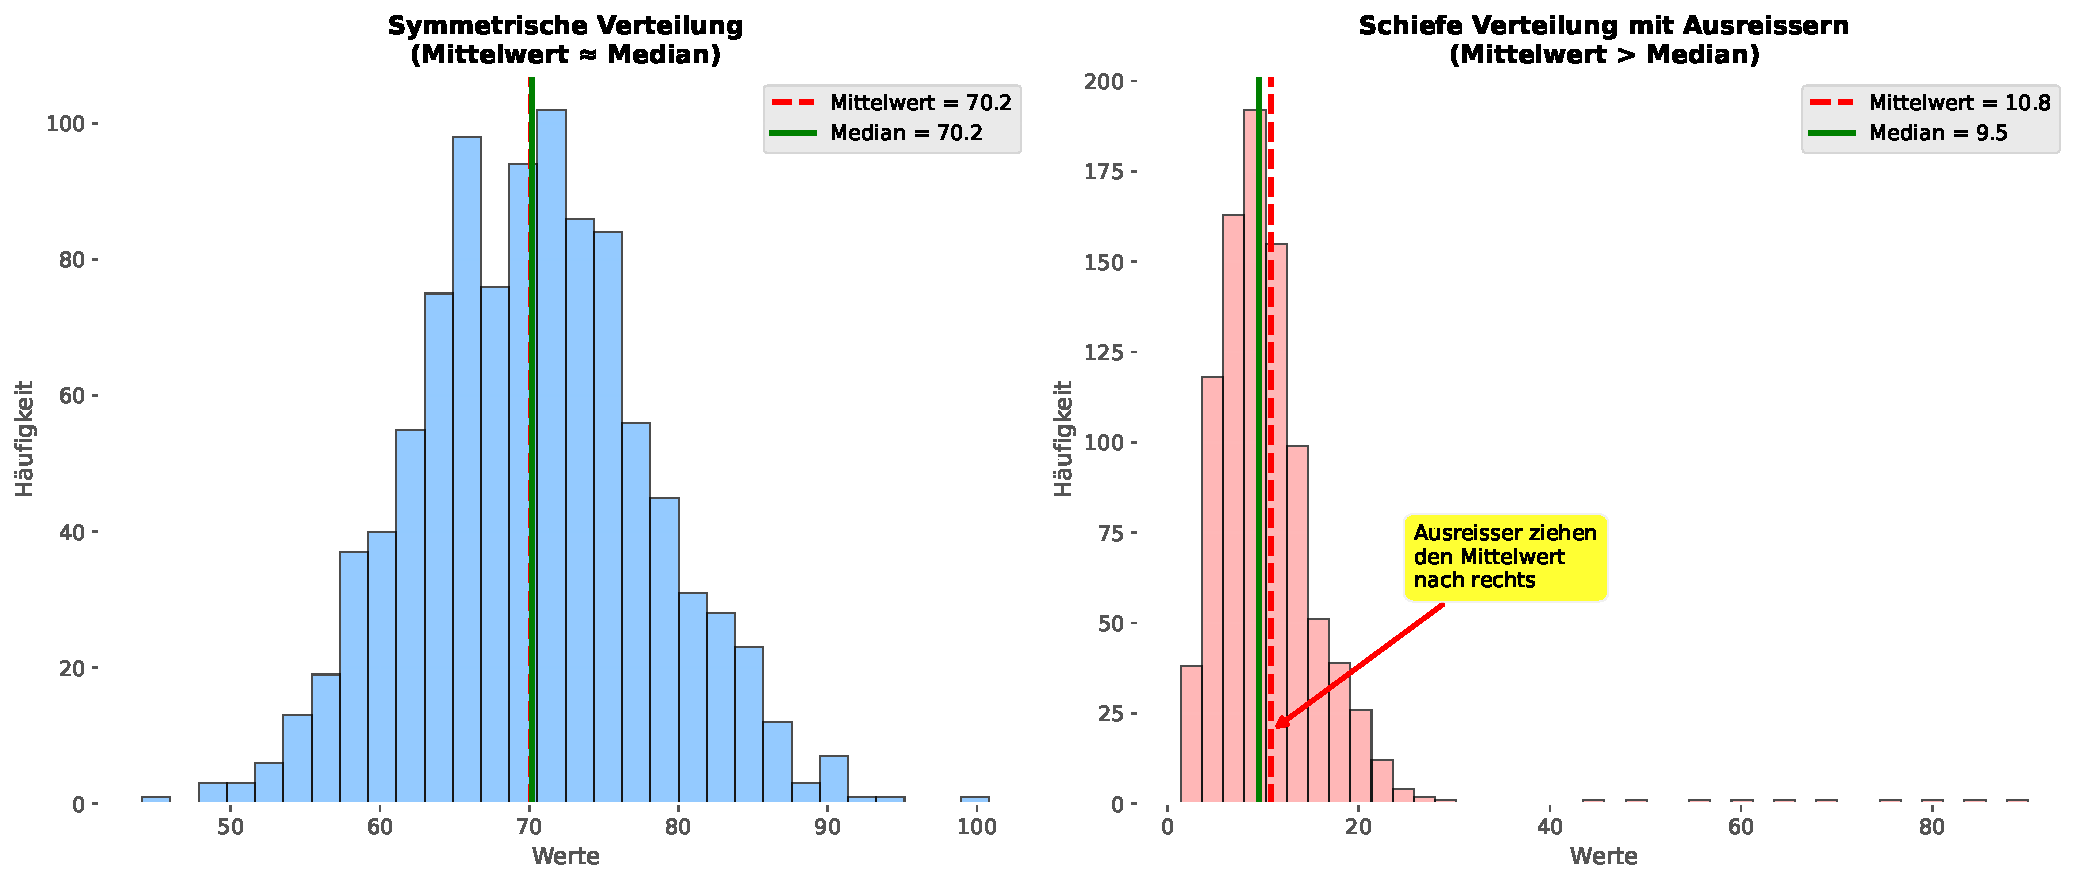
\includegraphics[width=0.95\textwidth]{Various/Wahlpflichtmodul Statistik/Figures/plots_mean_vs_median.pdf}
    \end{figure}
    \begin{itemize}
        \item \textbf{Links}: Symmetrisch $\Rightarrow$ Mittelwert $\approx$ Median
        \item \textbf{Rechts}: Schief mit Ausreissern $\Rightarrow$ Mittelwert $>$ Median
    \end{itemize}
\end{frame}

\begin{frame}{Beispiel: Taschengeld mit Ausreisser}
    \textbf{Daten} (monatliches Taschengeld in \gls{CHF}): 20, 25, 25, 30, 30, 35, 40, 400

    \vspace{0.5em}
    \begin{figure}[H]
        \centering
        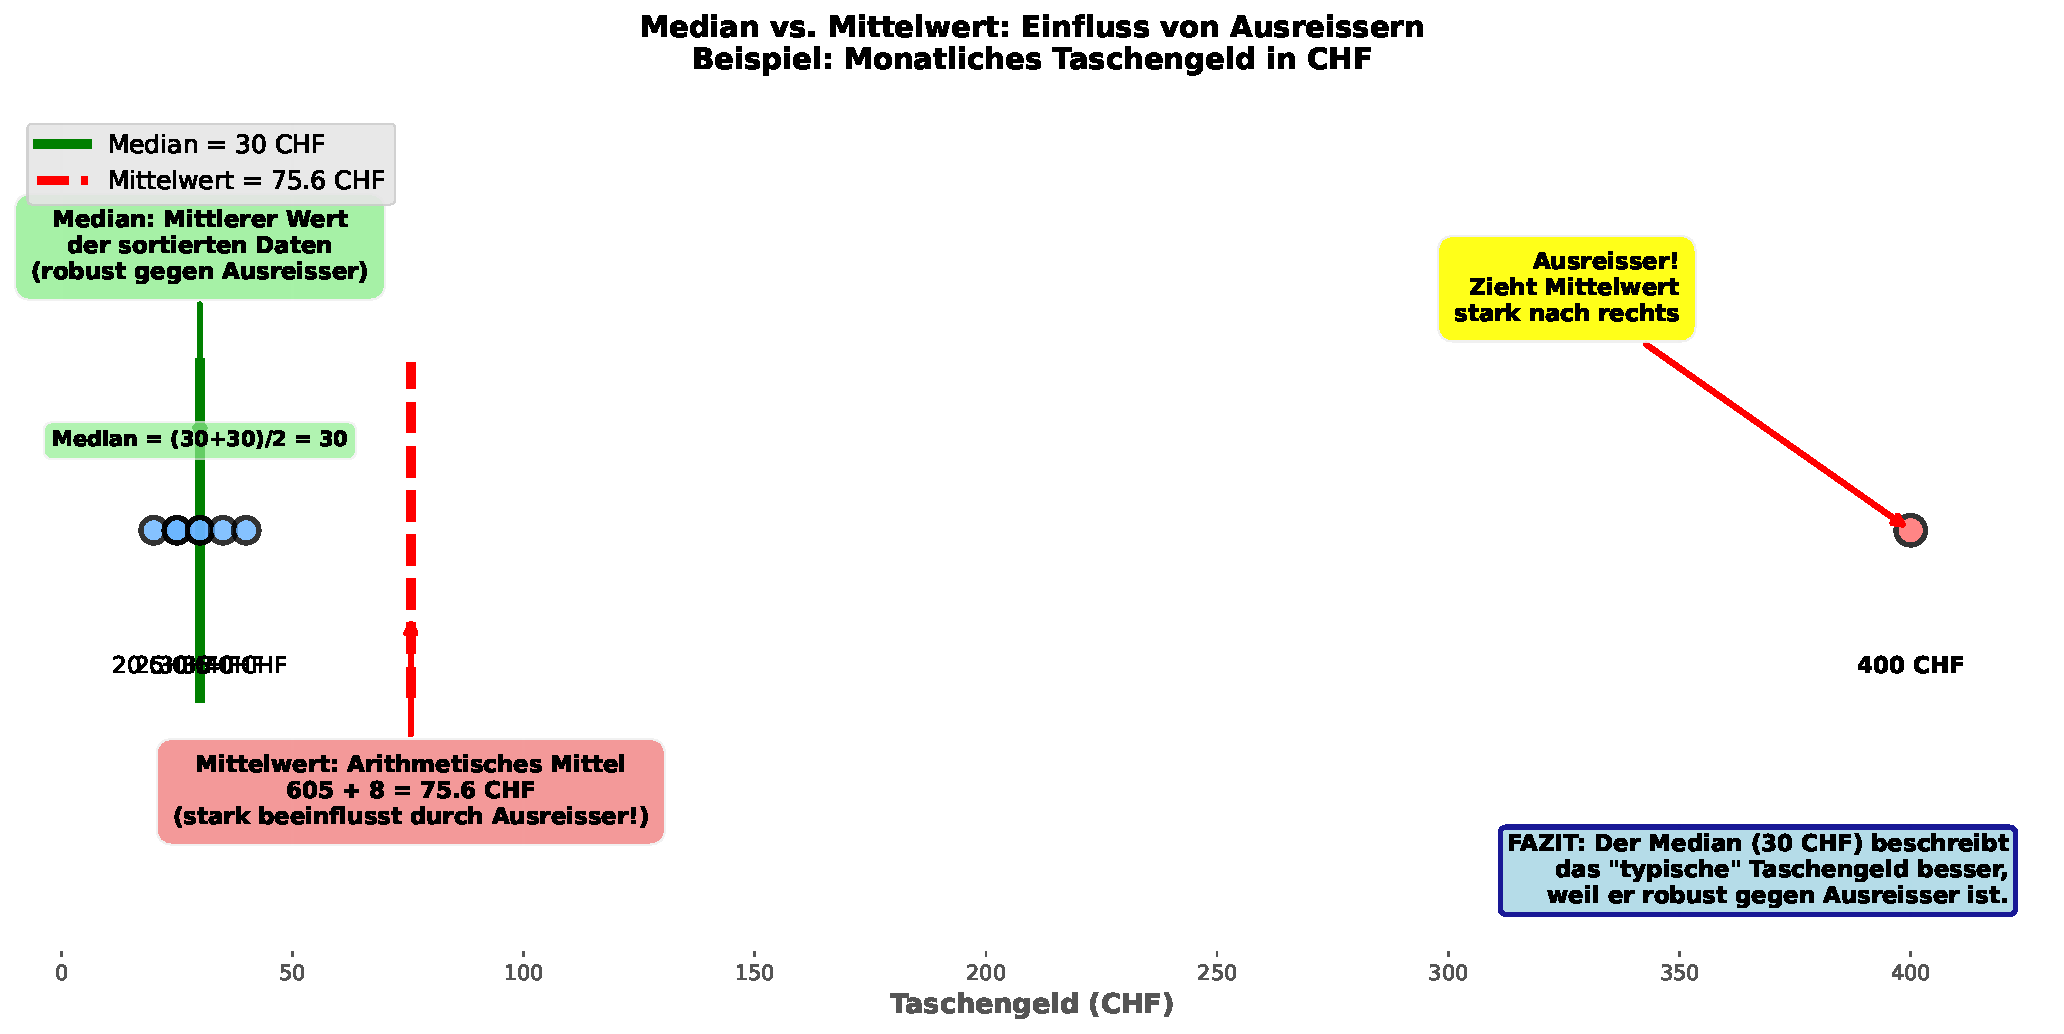
\includegraphics[width=0.85\textwidth]{Various/Wahlpflichtmodul Statistik/Figures/plots_median_calculation.pdf}
    \end{figure}
\end{frame}

\begin{frame}{Streuung: Wie stark variieren die Daten?}
    \begin{itemize}[<+->]
        \item \textbf{Spannweite}: $\max(x) - \min(x)$
              \begin{itemize}
                  \item Einfach, aber stark von Extremwerten abhängig
              \end{itemize}
        \item \textbf{Interquartilsabstand (\gls{IQR})}: $Q3 - Q1$
              \begin{itemize}
                  \item Mittlere 50\% der Daten
                  \item Robust gegen Ausreisser
              \end{itemize}
        \item \textbf{Standardabweichung (\gls{SD})}:
              \[
                  s = \sqrt{\frac{1}{n-1}\sum_{i=1}^{n}(x_i-\bar{x})^2}
              \]
              \begin{itemize}
                  \item Misst durchschnittliche Abweichung vom Mittelwert
                  \item Reagiert auf Ausreisser
              \end{itemize}
    \end{itemize}

    \vspace{0.5em}
    \only<4>{
        \begin{block}{Typische Paarungen}
            Median + \gls{IQR} \quad oder \quad Mittelwert + \gls{SD}
        \end{block}
    }
\end{frame}

\begin{frame}{Quartile: Daten in vier Teile teilen}
    \begin{figure}[H]
        \centering
        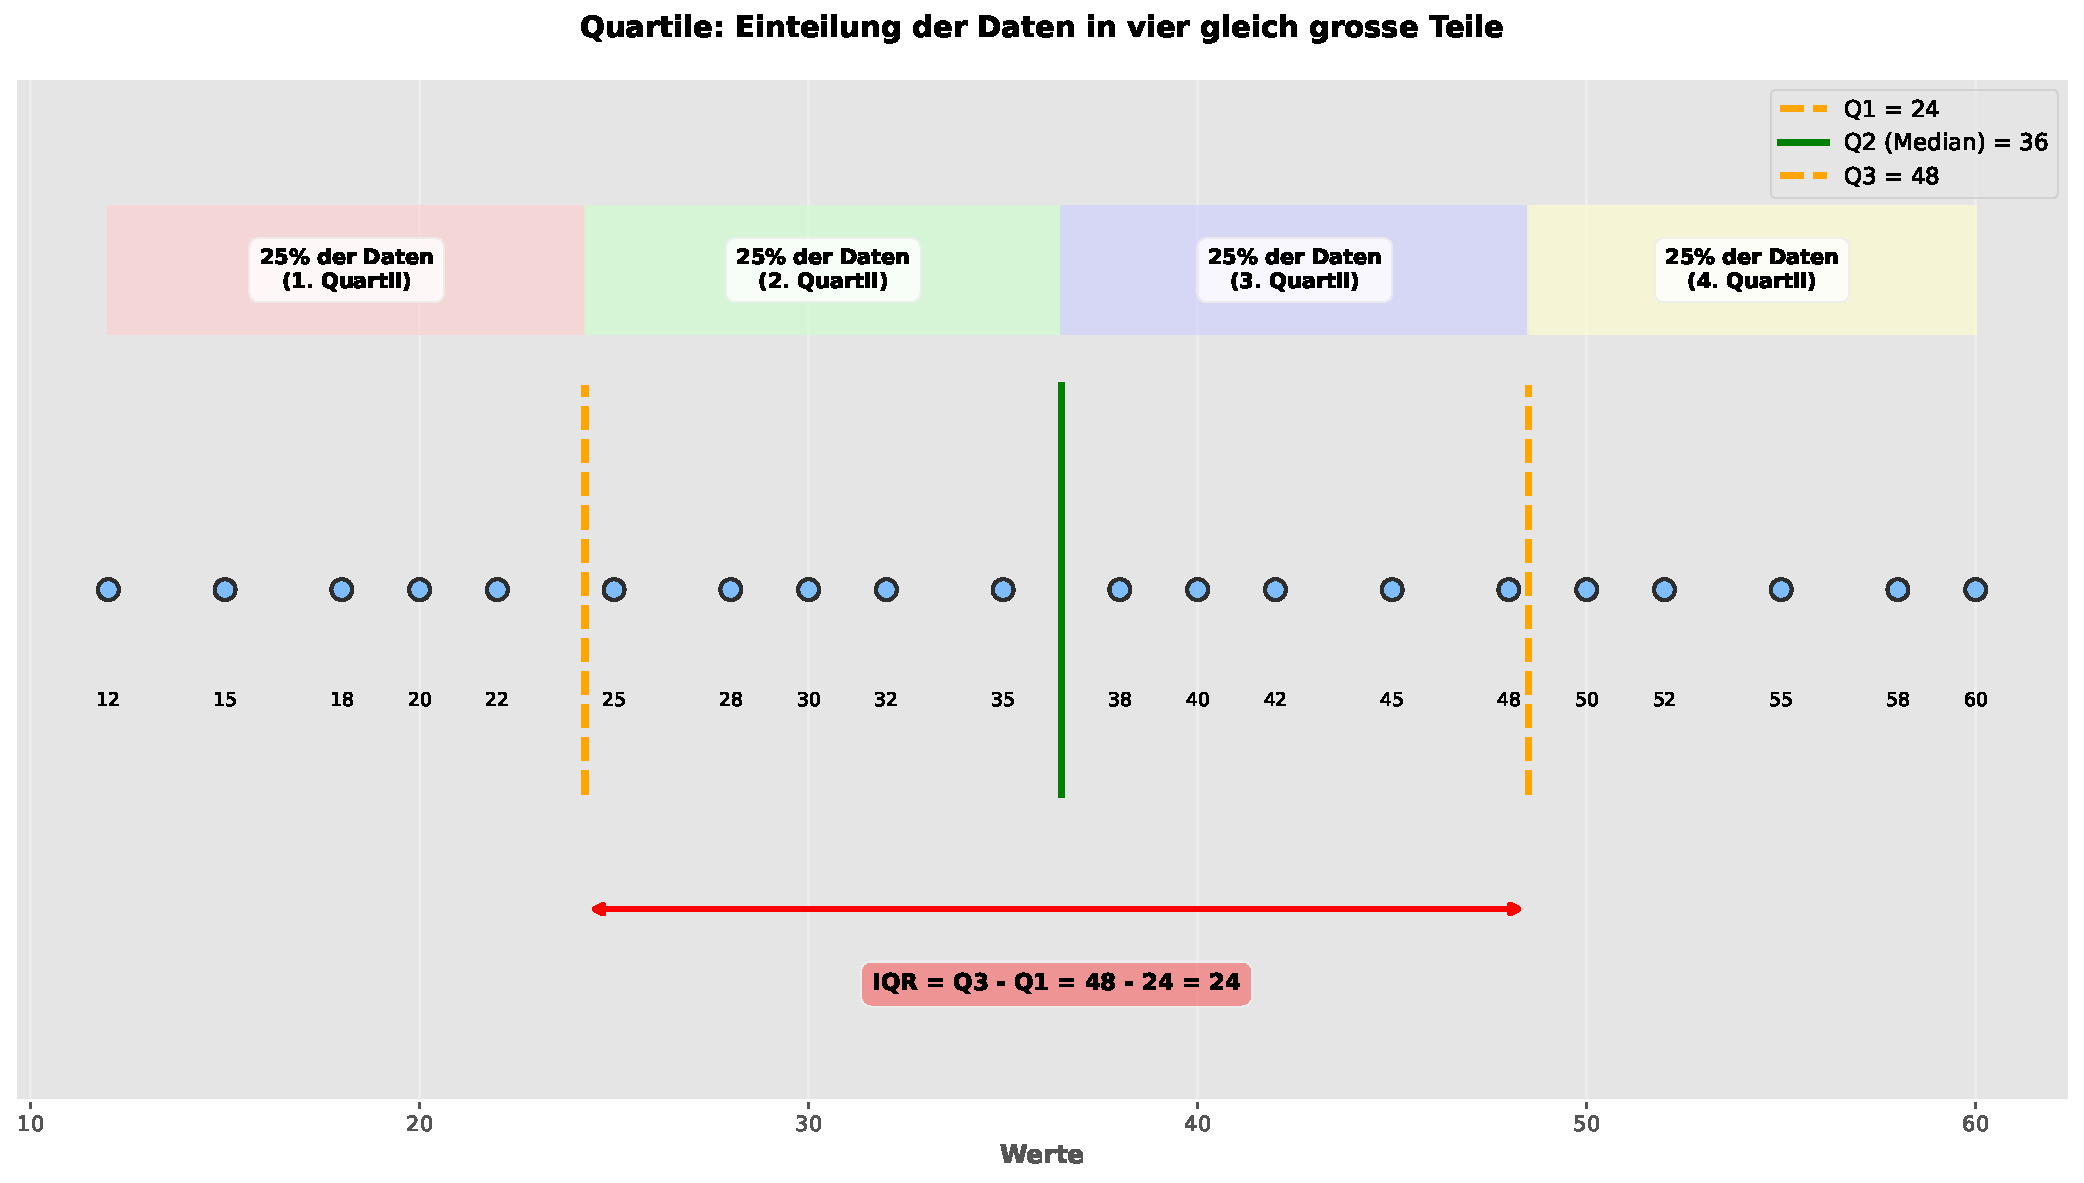
\includegraphics[width=0.95\textwidth]{Various/Wahlpflichtmodul Statistik/Figures/plots_quartiles.pdf}
    \end{figure}
    \begin{itemize}
        \item Q1 = 25\%-Quantil, Q2 = Median, Q3 = 75\%-Quantil
        \item \gls{IQR} = Q3 - Q1 (mittlere 50\% der Daten)
    \end{itemize}
\end{frame}

\begin{frame}{Standardabweichung bei Normalverteilung}
    \begin{figure}[H]
        \centering
        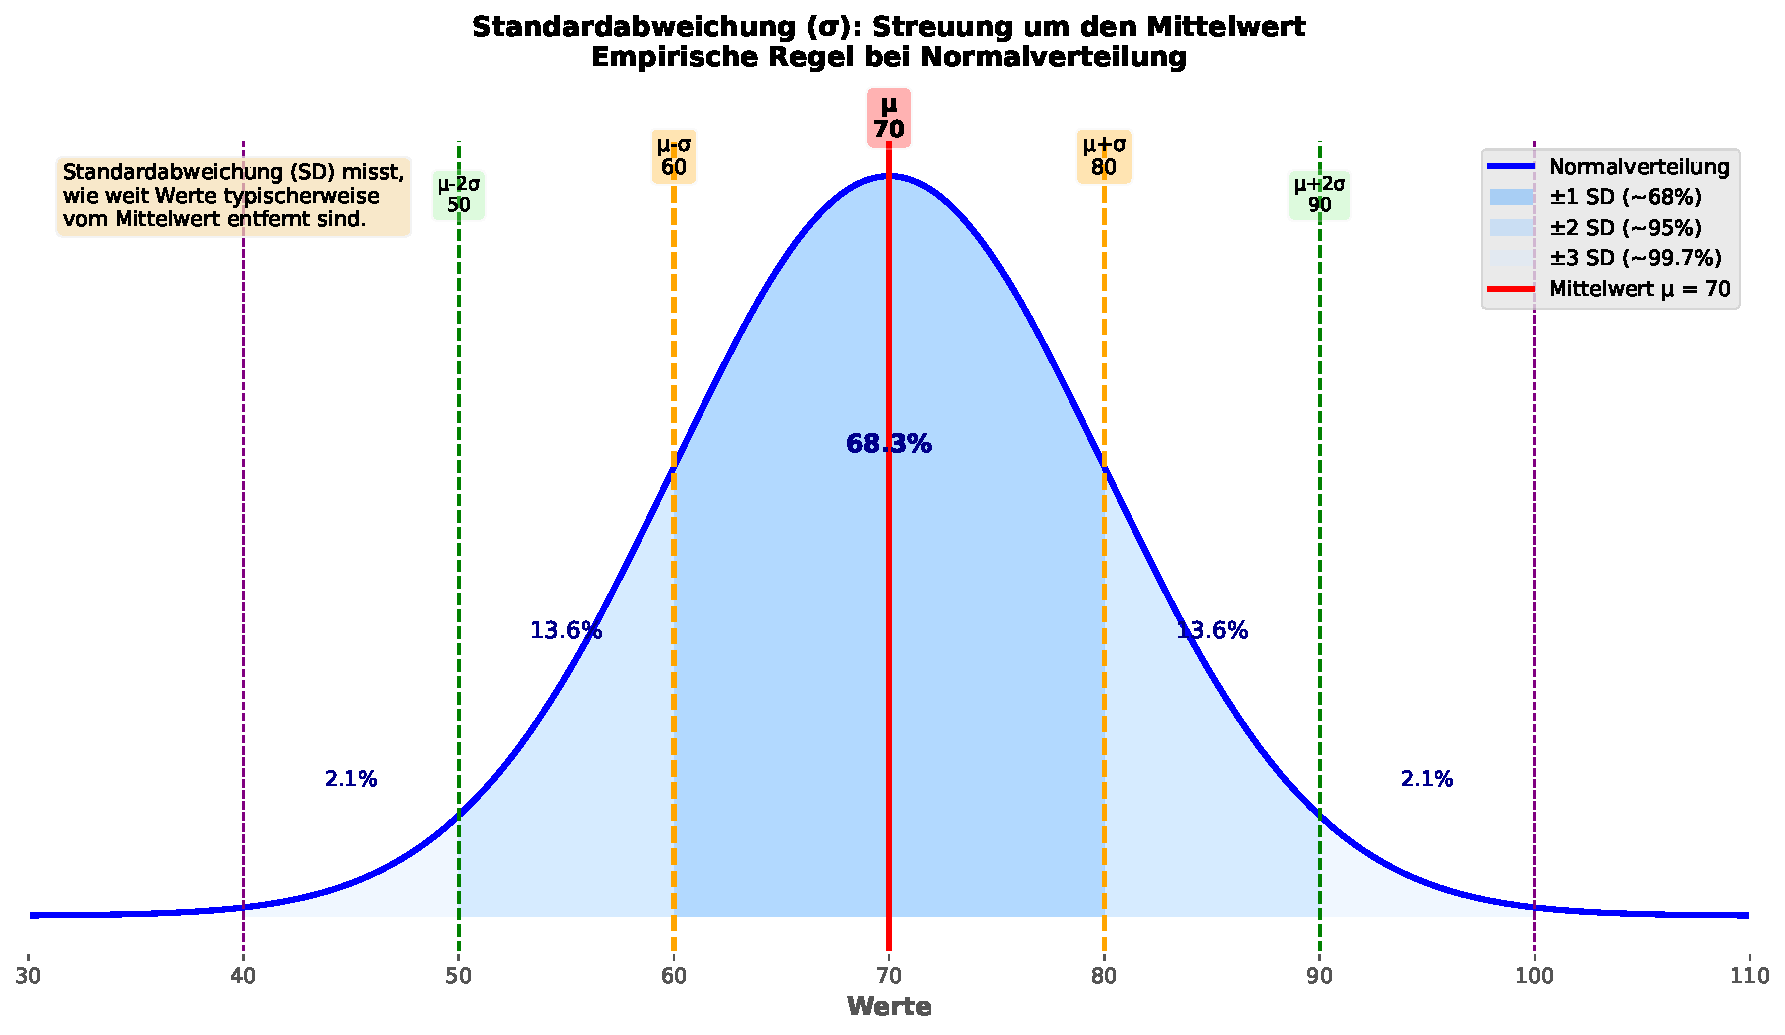
\includegraphics[width=0.9\textwidth]{Various/Wahlpflichtmodul Statistik/Figures/plots_standard_deviation.pdf}
    \end{figure}
    \begin{itemize}
        \item \textbf{68\%} der Daten liegen innerhalb von $\pm 1$ \gls{SD}
        \item \textbf{95\%} innerhalb von $\pm 2$ \gls{SD}
        \item \textbf{99.7\%} innerhalb von $\pm 3$ \gls{SD}
    \end{itemize}
\end{frame}

\begin{frame}{Übungen im Skript: Lage und Streuung}
    \begin{itemize}
        \item \aufgabebox{1.2 Median vs. Mittelwert mit Ausreisser}
    \end{itemize}
\end{frame}

\begin{frame}{Visualisierung: Scatterplot}
    \begin{minipage}[c]{0.58\linewidth}
        \begin{figure}[H]
            \centering
            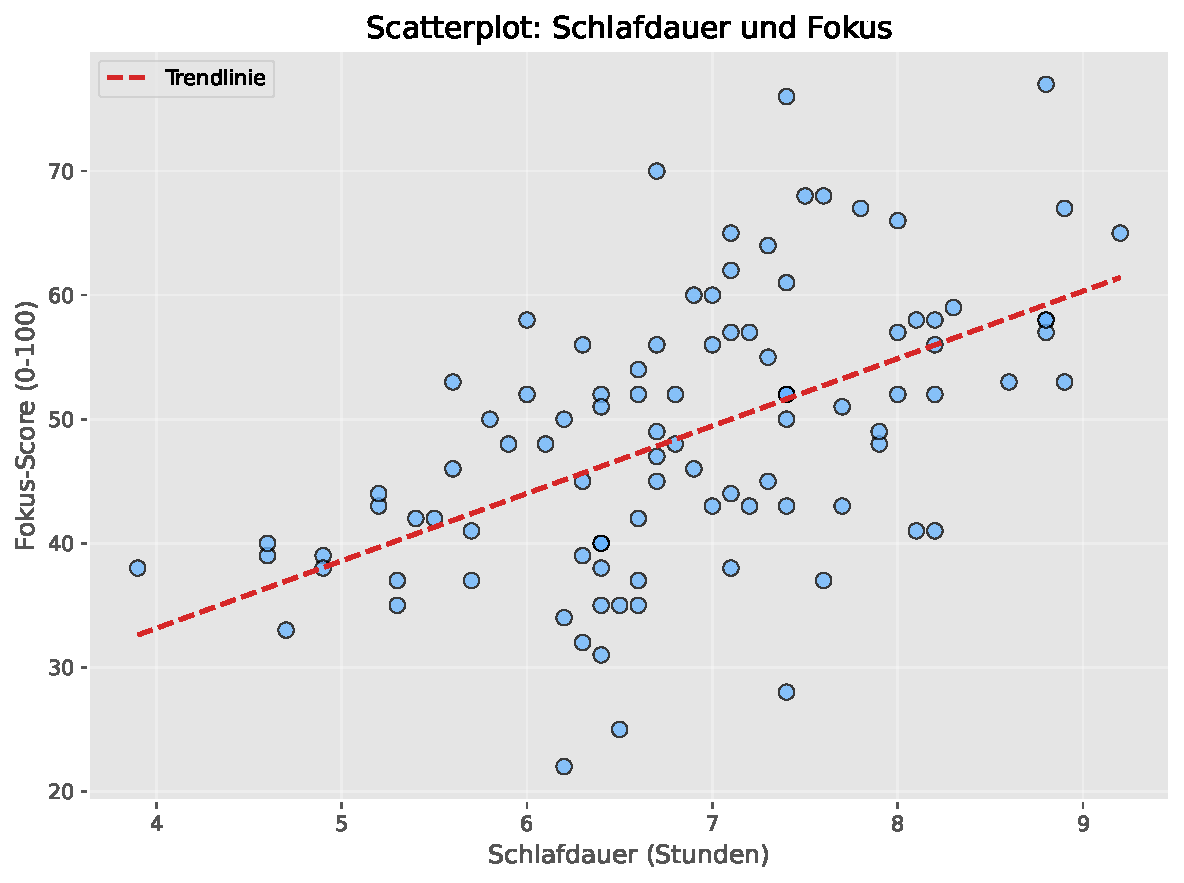
\includegraphics[width=\textwidth]{Various/Wahlpflichtmodul Statistik/Figures/plots_scatterplot.pdf}
        \end{figure}
    \end{minipage}\hfill
    \begin{minipage}[c]{0.38\linewidth}
        \textbf{Scatterplot}:
        \begin{itemize}
            \item Beziehung zwischen zwei metrischen Variablen
            \item Jeder Punkt = eine Beobachtung
            \item Zeigt Muster und Korrelationen
        \end{itemize}
    \end{minipage}
\end{frame}


\begin{frame}{Visualisierung: Balken- und Kreisdiagramm}
    \begin{minipage}[c]{0.60\linewidth}
        \begin{figure}[H]
            \centering
            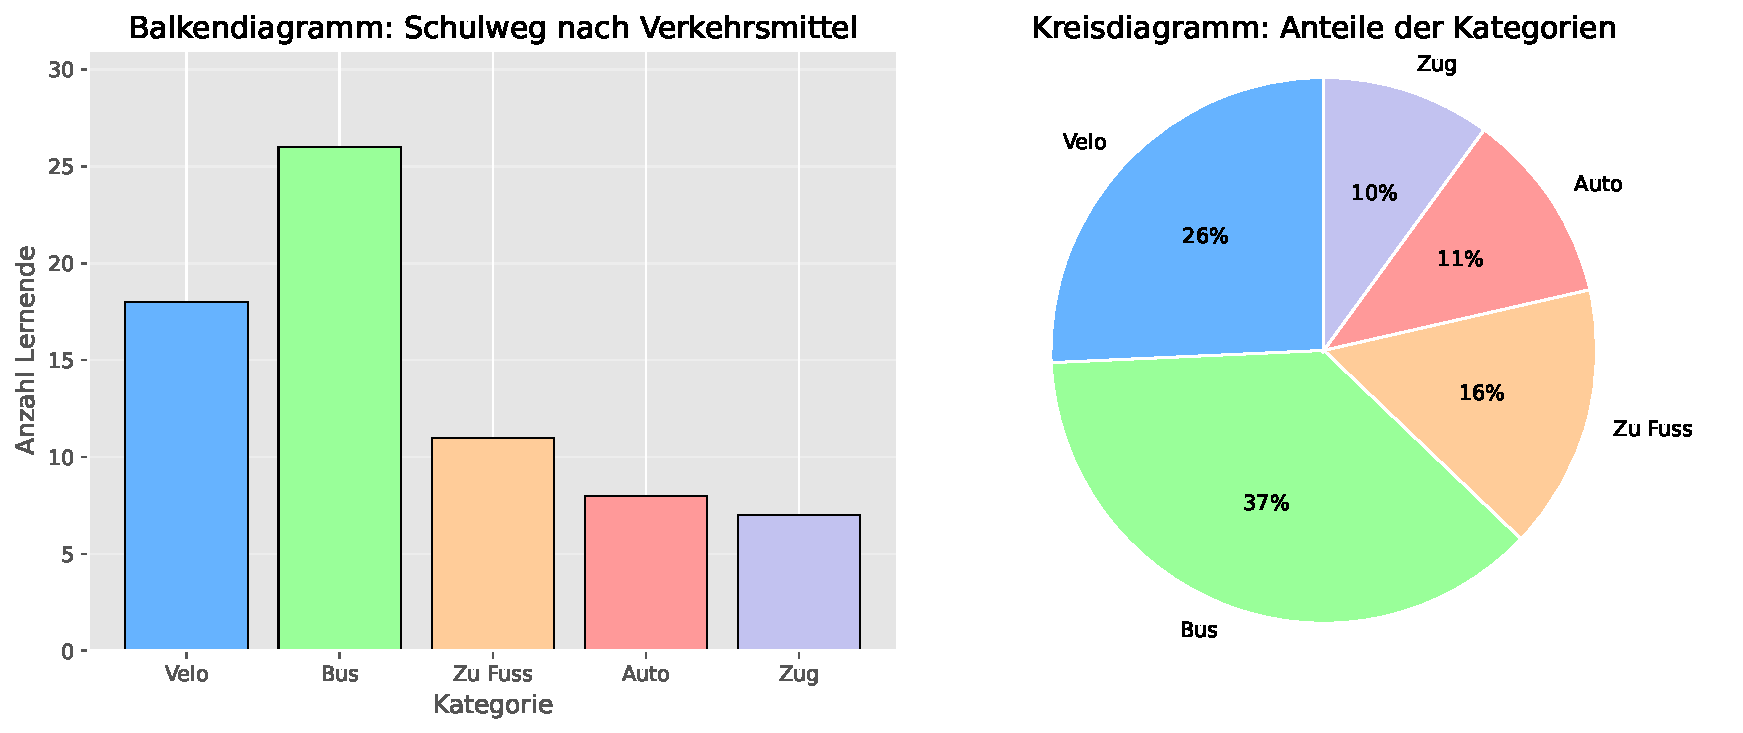
\includegraphics[width=\textwidth]{Various/Wahlpflichtmodul Statistik/Figures/plots_bar_pie.pdf}
        \end{figure}
    \end{minipage}\hfill
    \begin{minipage}[c]{0.36\linewidth}
        \begin{itemize}
            \item Für Kategorien (nominal)
            \item \textbf{Balken}: gut für Vergleiche und genaue Werte
            \item \textbf{Kreis}: nur bei wenigen Kategorien sinnvoll
        \end{itemize}
    \end{minipage}
\end{frame}

\begin{frame}{Visualisierung: Histogramm}
    \begin{minipage}[c]{0.48\linewidth}
        \begin{figure}[H]
            \centering
            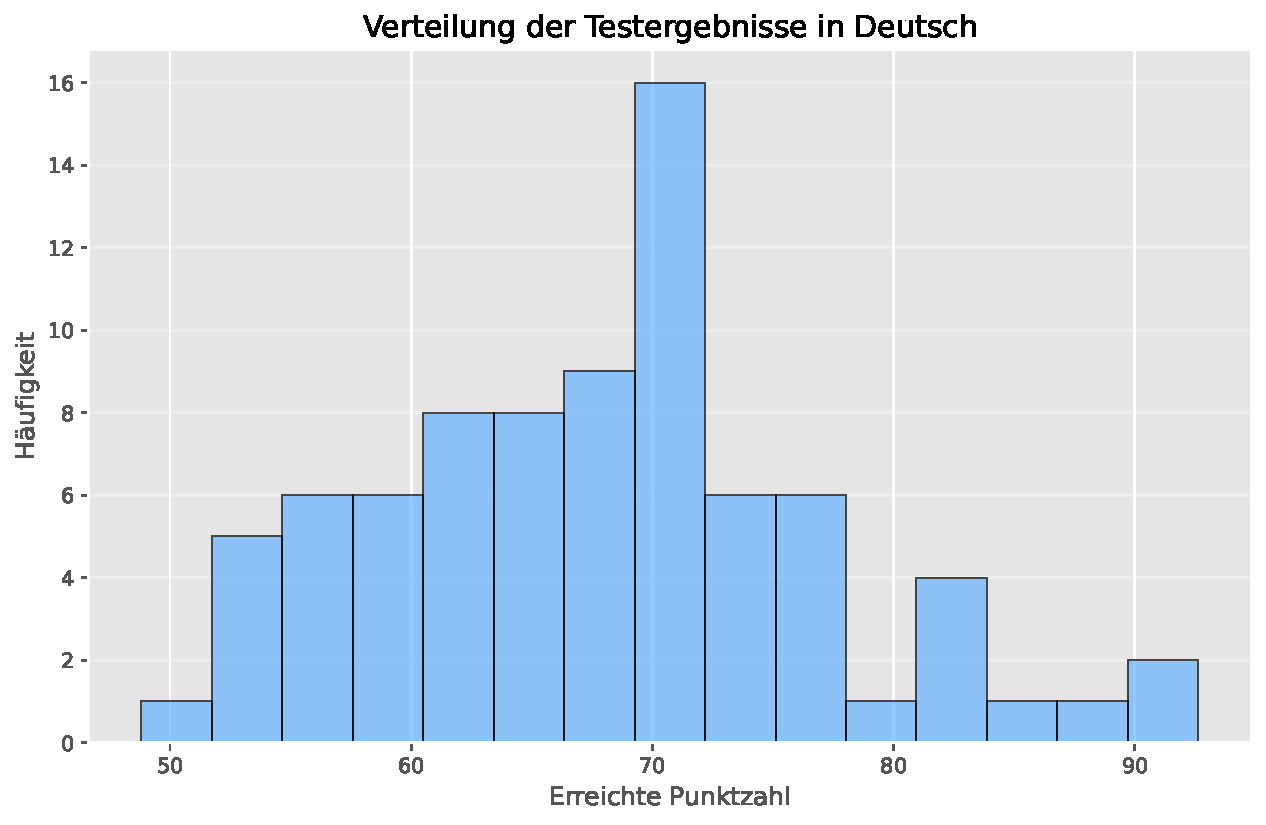
\includegraphics[width=\textwidth]{Various/Wahlpflichtmodul Statistik/Figures/plots_histogram.pdf}
        \end{figure}
    \end{minipage}\hfill
    \begin{minipage}[c]{0.48\linewidth}
        \textbf{Histogramm}:
        \begin{itemize}
            \item Zeigt Verteilung von Daten
            \item Für metrische Variablen
            \item Balken = Häufigkeit in Intervallen
            \item Zeigt Form der Verteilung
        \end{itemize}
    \end{minipage}
\end{frame}

\begin{frame}{Visualisierung: Boxplot}
    \begin{minipage}[c]{0.48\linewidth}
        \begin{figure}[H]
            \centering
            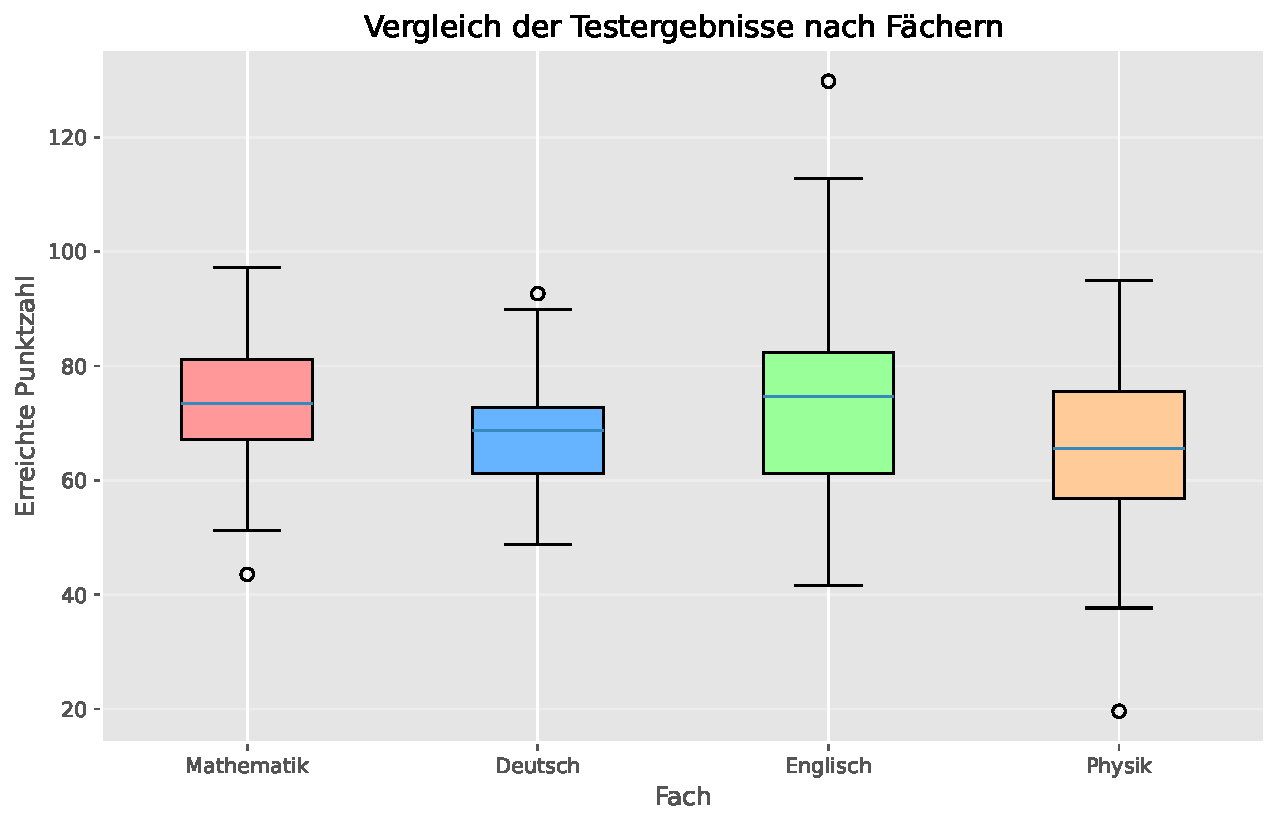
\includegraphics[width=\textwidth]{Various/Wahlpflichtmodul Statistik/Figures/plots_boxplot.pdf}
        \end{figure}
    \end{minipage}\hfill
    \begin{minipage}[c]{0.48\linewidth}
        \textbf{Boxplot}:
        \begin{itemize}
            \item Kompakte Darstellung
            \item Zeigt Median, Q1, Q3
            \item Whiskers = Datenbereich
            \item Punkte = Ausreisser
            \item Gut zum Vergleichen
        \end{itemize}
    \end{minipage}
\end{frame}

\begin{frame}{Boxplot: Anatomie}
    \begin{figure}[H]
        \centering
        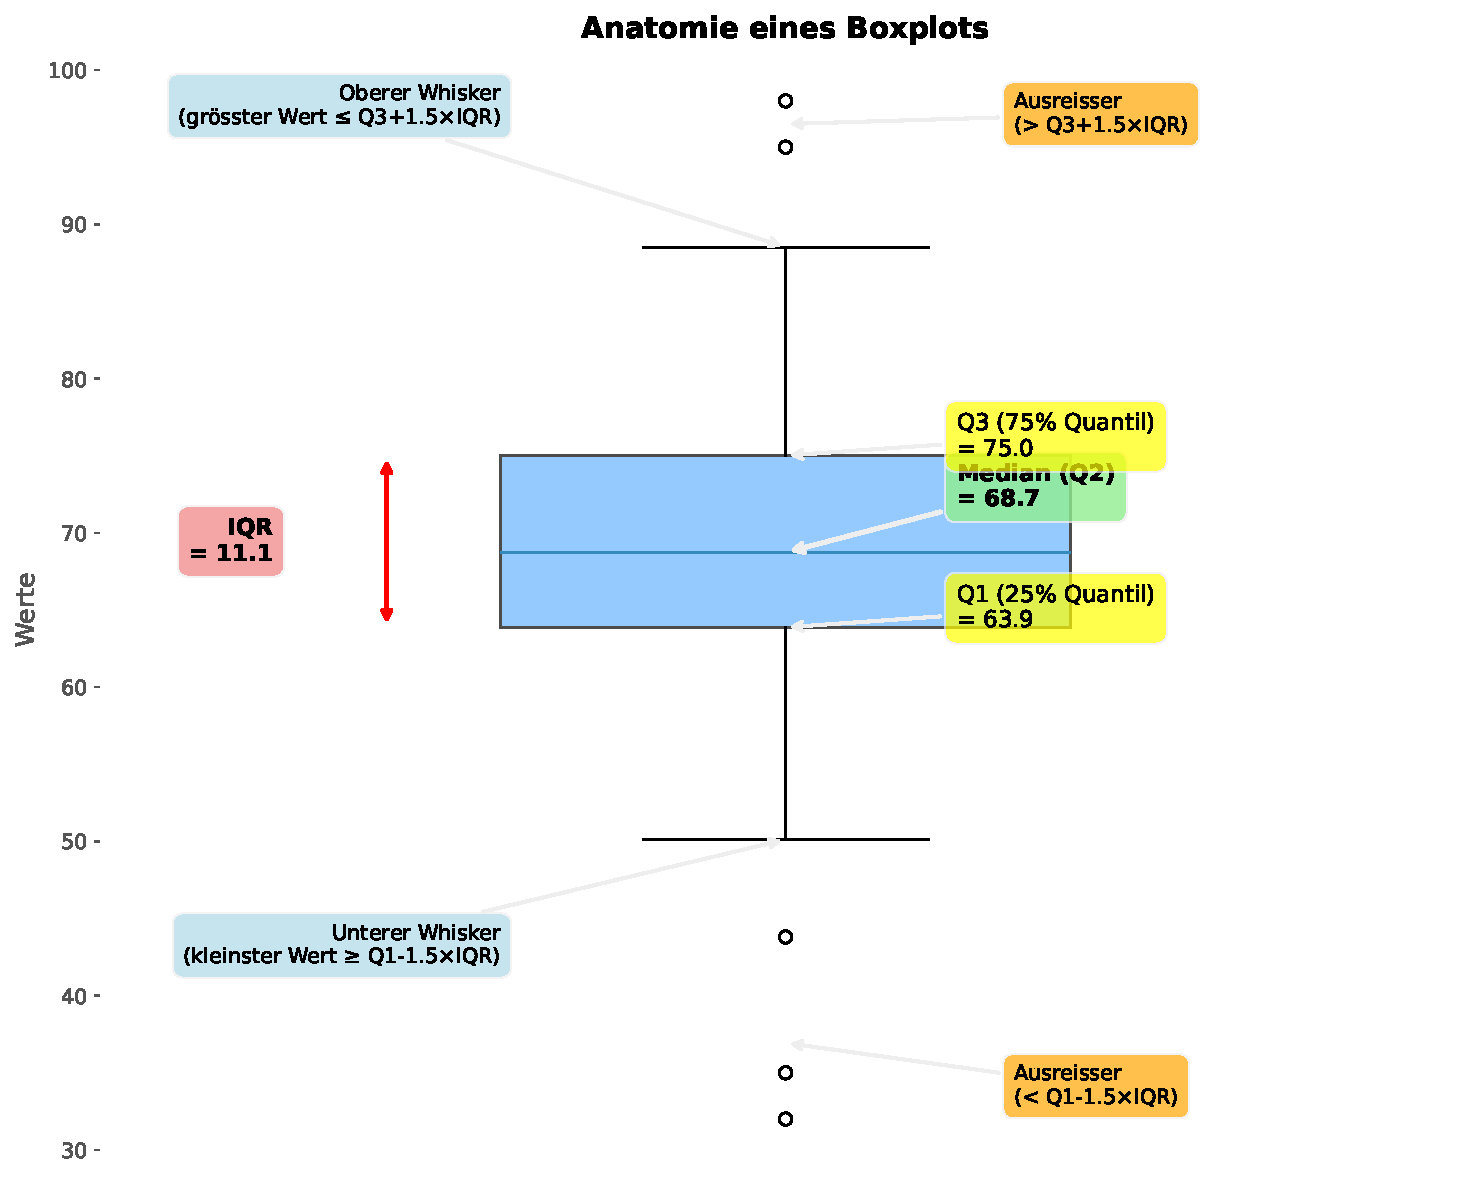
\includegraphics[width=0.75\textwidth]{Various/Wahlpflichtmodul Statistik/Figures/plots_boxplot_anatomy.pdf}
    \end{figure}
\end{frame}

\begin{frame}{Verteilungsformen}
    \begin{figure}[H]
        \centering
        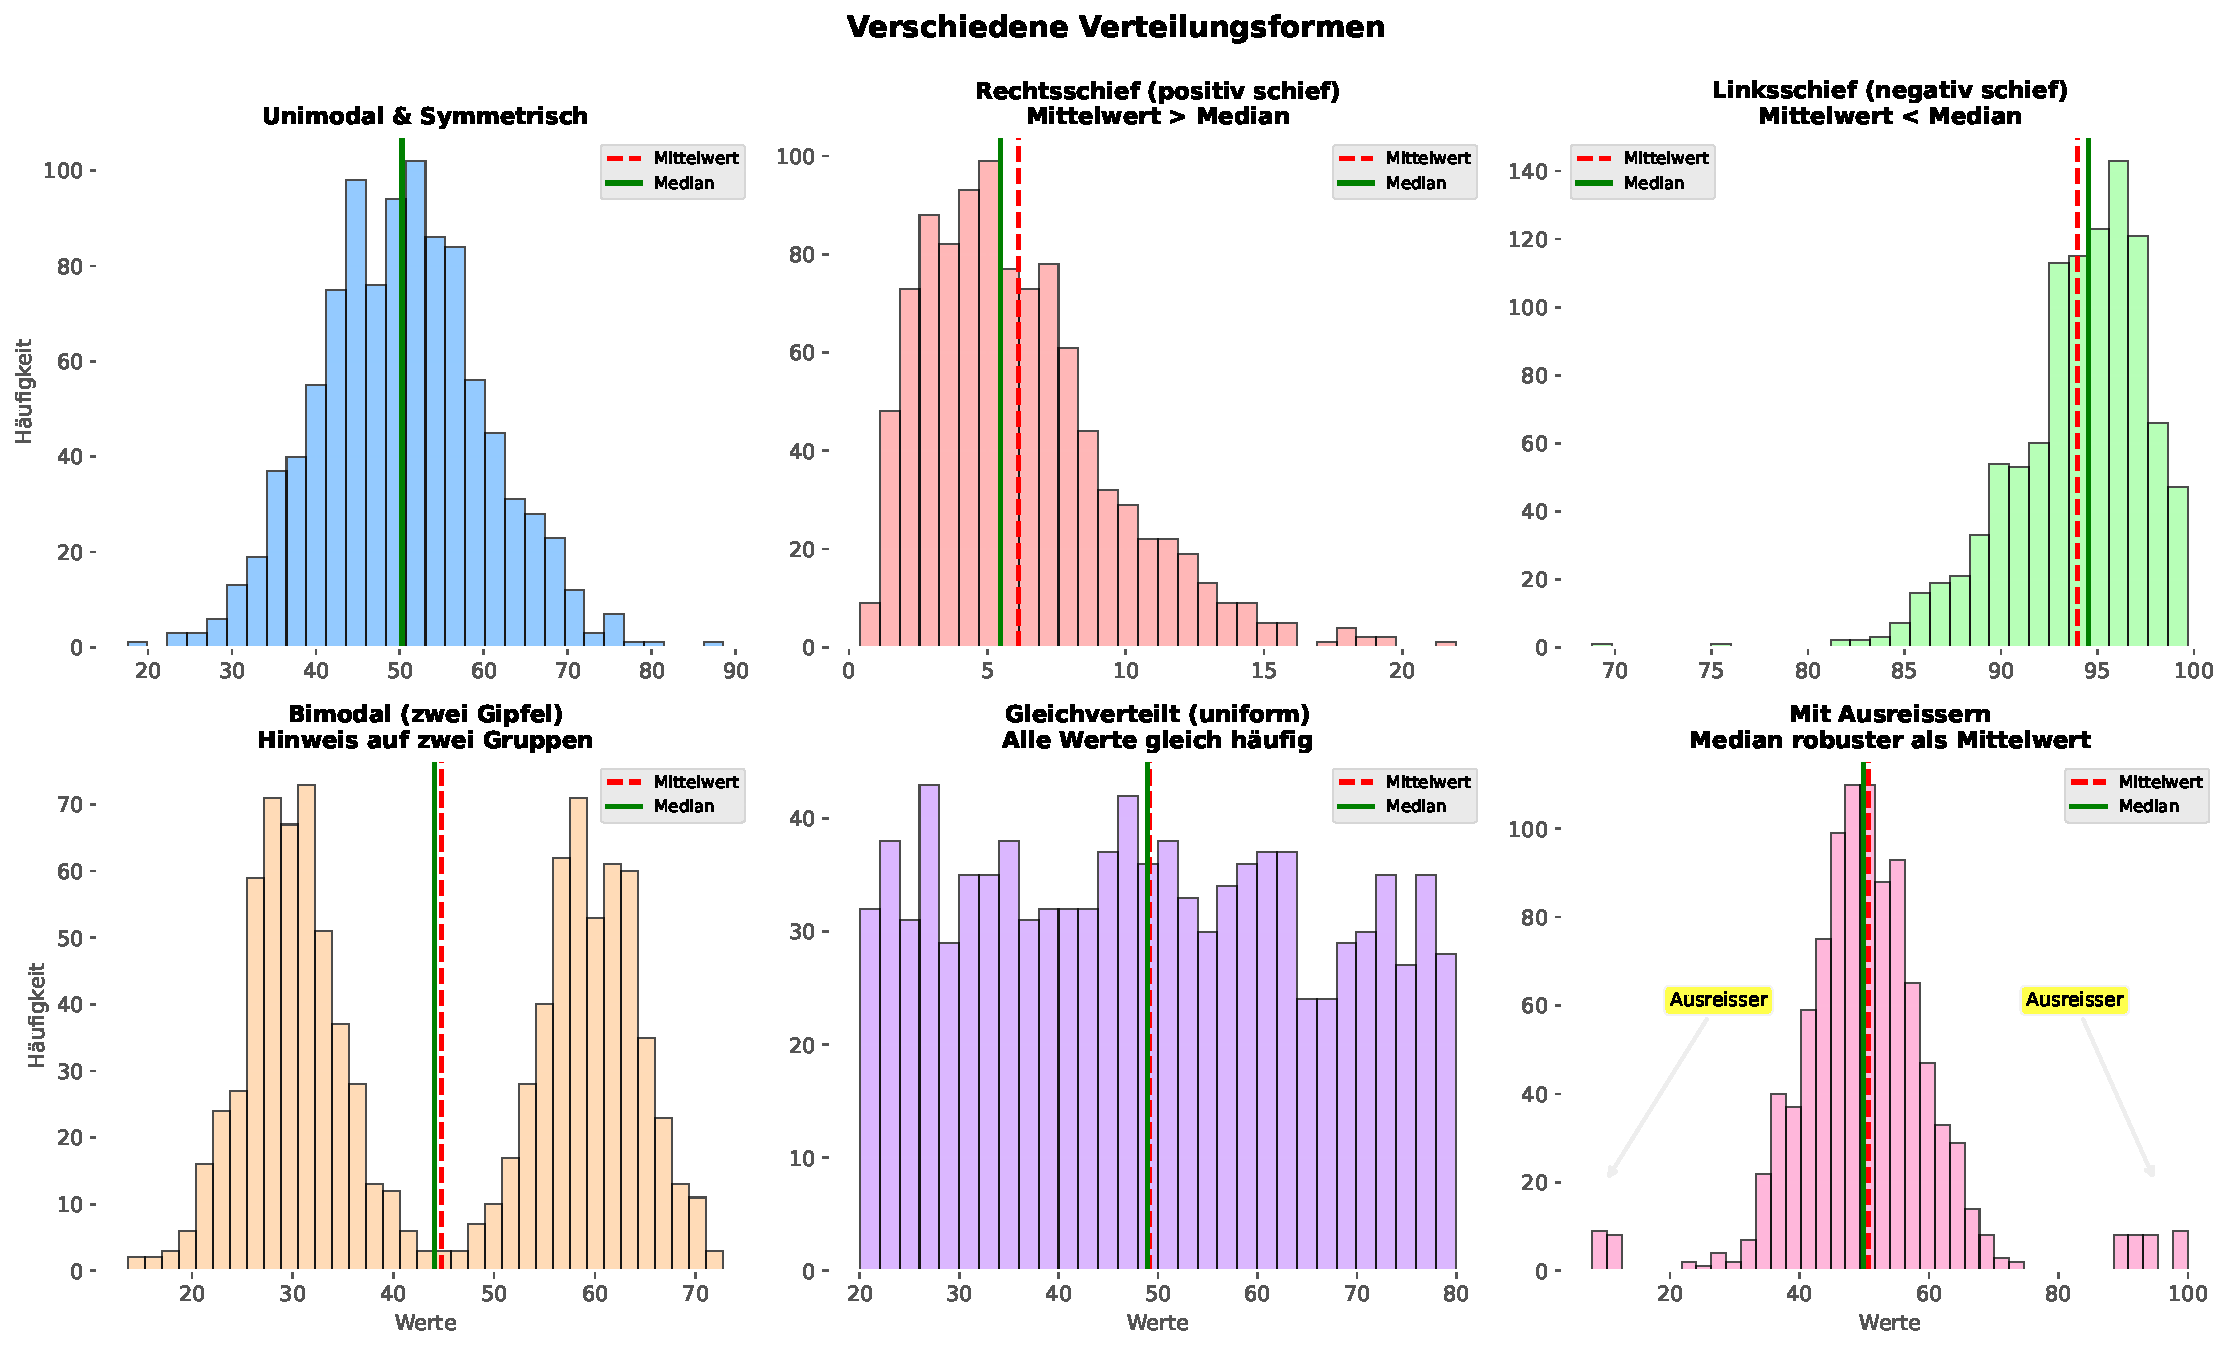
\includegraphics[width=0.95\textwidth]{Various/Wahlpflichtmodul Statistik/Figures/plots_distribution_shapes.pdf}
    \end{figure}
\end{frame}

\begin{frame}{Verteilungsformen: Interpretation}
    \begin{itemize}[<+->]
        \item \textbf{Symmetrisch}: Mittelwert $\approx$ Median
              \begin{itemize}
                  \item Daten gleichmässig um die Mitte verteilt
              \end{itemize}
        \item \textbf{Rechtsschief}: Mittelwert $>$ Median
              \begin{itemize}
                  \item Wenige hohe Ausreisser ziehen Mittelwert nach rechts
                  \item Beispiel: Einkommen, Immobilienpreise
              \end{itemize}
    \end{itemize}

    \vspace{0.5em}
    \begin{block}{Reduktion im Modul}
        Wir fokussieren auf \textbf{symmetrisch} vs. \textbf{rechtsschief}, weil diese Unterscheidung für die Wahl von Kennzahlen am wichtigsten ist.
    \end{block}
\end{frame}

% \begin{frame}{Vorsicht: Irreführende Grafiken!}
%     \begin{figure}[H]
%         \centering
%         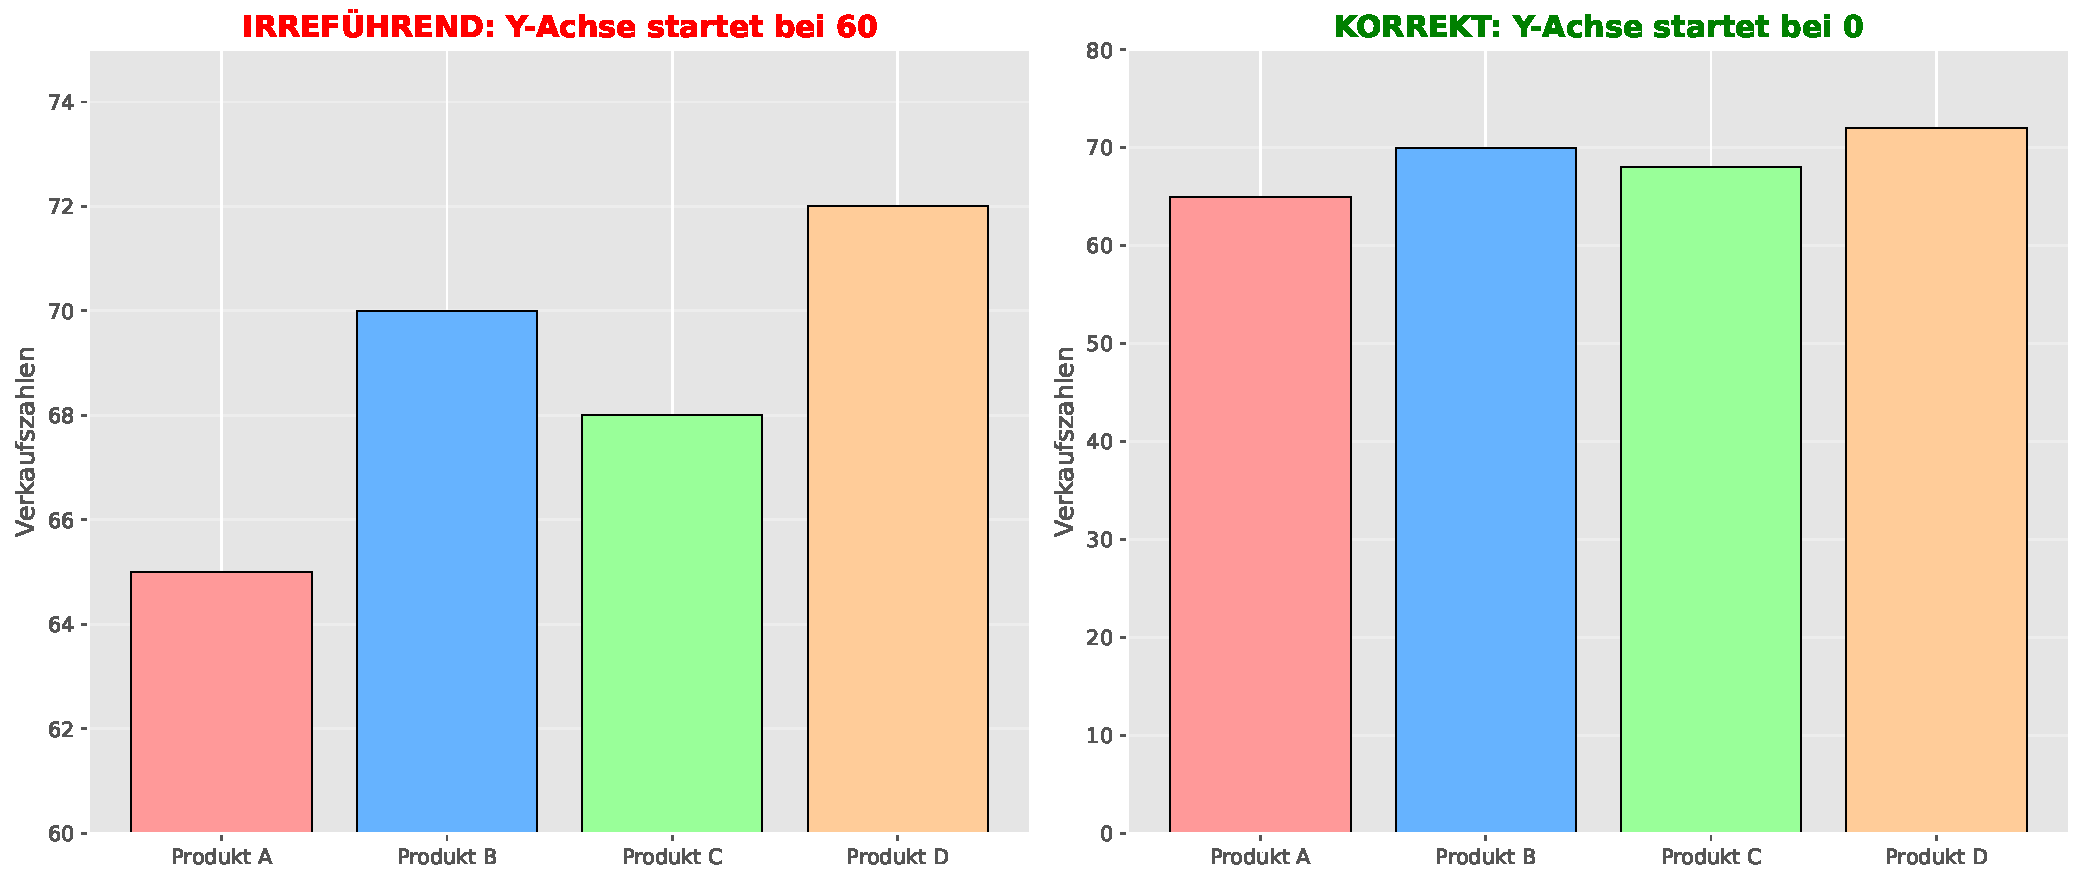
\includegraphics[width=0.9\textwidth]{Various/Wahlpflichtmodul Statistik/Figures/plots_misleading_axes.pdf}
%     \end{figure}

%     \begin{alertblock}{Checkliste beim Lesen von Grafiken}
%         \begin{itemize}
%             \item Startet die Achse bei 0?
%             \item Sind Kategorien gleich breit?
%             \item Fehlen Werte oder Gruppen?
%         \end{itemize}
%     \end{alertblock}
% \end{frame}

\begin{frame}{Übungen im Skript: Diagramme lesen}
    \begin{itemize}
        \item \aufgabebox{1.3 Irreführende Achsen erkennen}
    \end{itemize}
\end{frame}

\begin{frame}{Korrelation $\neq$ Kausalität}
    \begin{alertblock}{Wichtigste Regel}
        \textbf{Korrelation bedeutet nicht Kausalität!}
    \end{alertblock}

    \vspace{1em}
    \textbf{Warum keine sichere Ursache-Wirkung-Aussage?}
    \begin{itemize}[<+->]
        \item \textbf{Drittvariablen}: Eine versteckte Variable beeinflusst beide
              \begin{itemize}
                  \item Beispiel: Eis-Verkauf und Badeunfälle (beide durch Temperatur)
              \end{itemize}
        \item \textbf{Umgekehrte Kausalität}: Y könnte X beeinflussen
        \item \textbf{Zufall}: Bei kleinen Stichproben können zufällige Muster entstehen
        \item \textbf{Messfehler}: Ungenaue oder verzerrte Datenerhebung
    \end{itemize}
\end{frame}

\begin{frame}{Schliessende Statistik: Grundidee}
    \begin{itemize}[<+->]
        \item \textbf{Beschreibend}: Was zeigt unsere Stichprobe?
        \item \textbf{Schliessend}: Was lässt sich über eine grössere Grundgesamtheit sagen?
        \item Zentral ist die Frage nach \textbf{Unsicherheit} und \textbf{Zufall}
    \end{itemize}

    \vspace{0.8em}
    \begin{block}{Begriffe}
        Stichprobe = beobachtete Teilmenge, Grundgesamtheit = Zielgruppe der Aussage
    \end{block}
\end{frame}

\begin{frame}{Vertrauensintervall und Signifikanz}
    \begin{itemize}[<+->]
        \item Ein 95\%-\textbf{Vertrauensintervall} gibt einen plausiblen Bereich für den echten Effekt an
        \item Für Anteilsdifferenzen nutzen wir
              \[
                  \hat{\Delta} \pm 1.96\cdot \mathrm{SE}(\hat{\Delta})
              \]
              mit
              \[
                  \mathrm{SE}(\hat{\Delta})=\sqrt{\frac{\hat{p}_{\mathrm{exp}}(1-\hat{p}_{\mathrm{exp}})}{n_{\mathrm{exp}}}+\frac{\hat{p}_{\mathrm{kontr}}(1-\hat{p}_{\mathrm{kontr}})}{n_{\mathrm{kontr}}}}
              \]
        \item Bei einem Unterschied ist 0 die Referenz für \enquote{kein Unterschied}
        \item 0 ausserhalb Intervall \Rightarrow systematischer Unterschied plausibel
        \item 0 im Intervall \Rightarrow \enquote{kein klarer Unterschied} bleibt vereinbar
        \item Signifikanztests und Vertrauensintervalle beruhen auf derselben Zufallslogik
    \end{itemize}
\end{frame}

\begin{frame}{Kontrollgruppen machen Vergleiche fair}
    \begin{itemize}[<+->]
        \item Ohne Kontrollgruppe werden Unterschiede oft zu schnell kausal interpretiert
        \item Mit Kontrollgruppe vergleichen wir gegen eine sinnvolle Referenz
        \item Beispiel: Lernritual vs. kein Lernritual
    \end{itemize}
\end{frame}

\begin{frame}{MythBusters-Idee: Ist Gähnen ansteckend?}
    \begin{figure}[H]
        \centering
        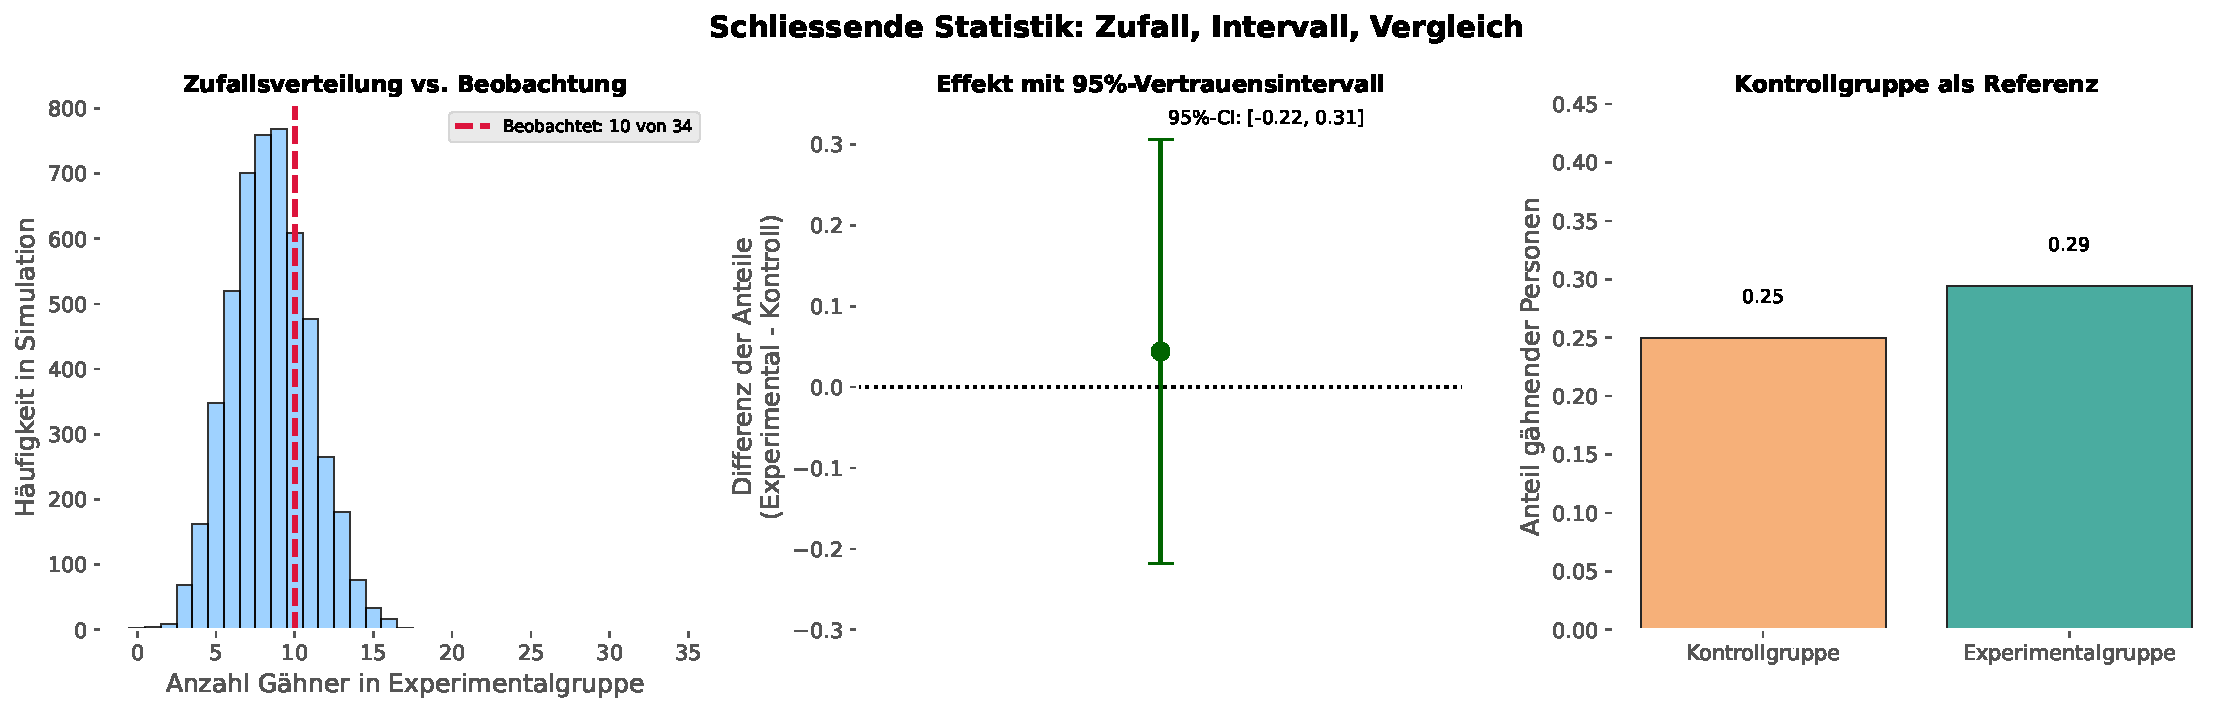
\includegraphics[width=0.95\textwidth]{Various/Wahlpflichtmodul Statistik/Figures/plots_inferential_basics.pdf}
    \end{figure}
    \begin{itemize}
        \item Daten: $24/40$ (Experimentalgruppe) vs. $14/40$ (Kontrollgruppe)
        \item Wir rechnen den Unterschied der Anteile Schritt für Schritt
        \item Ziel: Intervall bestimmen und 0 als Referenzwert prüfen
    \end{itemize}
\end{frame}

\begin{frame}{Gähn-Experiment: Durchgerechnetes Beispiel}
    \small
    \[
        \hat{p}_{\mathrm{exp}}=\frac{24}{40}=0.60,
        \qquad
        \hat{p}_{\mathrm{kontr}}=\frac{14}{40}=0.35
    \]
    \[
        \hat{\Delta}=\hat{p}_{\mathrm{exp}}-\hat{p}_{\mathrm{kontr}}=0.25
    \]
    \[
        \mathrm{SE}(\hat{\Delta})
        =\sqrt{\frac{0.60\cdot0.40}{40}+\frac{0.35\cdot0.65}{40}}
        =\sqrt{0.01169}\approx0.108
    \]
    \[
        95\%\text{-CI}=\hat{\Delta}\pm1.96\cdot\mathrm{SE}(\hat{\Delta})
        =0.25\pm1.96\cdot0.108
        =[0.038,0.462]
    \]
    \begin{block}{Interpretation}
        0 liegt nicht im Intervall \Rightarrow \enquote{kein Unterschied} ist mit den Daten nicht gut vereinbar.
    \end{block}
\end{frame}

\begin{frame}{Gähn-Experiment: Didaktischer Ablauf}
    \begin{enumerate}
        \item Anteile aus den Rohdaten berechnen
        \item Unterschied der Anteile als Effektgrösse bestimmen
        \item Standardfehler berechnen
        \item 95\%-Vertrauensintervall bestimmen
        \item 0-Regel interpretieren und Rolle der Kontrollgruppe begründen
    \end{enumerate}
\end{frame}

\begin{frame}{Kontingenztabelle: Kategoriale Daten}
    \textbf{Beispiel}: Musik beim Lernen vs. Lernmodus

    \vspace{0.5em}
    \begin{table}[H]
        \centering
        \begin{tabular}{l c c c}
            \toprule
                                & \textbf{Alleine} & \textbf{Gruppe} & \textbf{Summe} \\
            \midrule
            \textbf{Mit Musik}  & 45 (56\%)        & 25 (31\%)       & 70             \\
            \textbf{Ohne Musik} & 35 (44\%)        & 55 (69\%)       & 90             \\
            \textbf{Summe}      & 80               & 80              & 160            \\
            \bottomrule
        \end{tabular}
    \end{table}

    \vspace{0.5em}
    \begin{itemize}
        \item \textbf{Zulässig}: \enquote{In dieser Stichprobe hören mehr Einzellerner Musik}
        \item \textbf{Nicht zulässig}: \enquote{Musik verursacht besseres Lernen} (Kausalität!)
    \end{itemize}
\end{frame}


\begin{frame}{Übungen im Skript: Aufgabenpaket und Challenge}
    \begin{itemize}
        \item \aufgabebox{1.4: Kennzahlen interpretieren}
        \item \aufgabebox{1.5: Histogramm, Boxplot, Scatterplot}
        \item \challengebox{1.6: Kontingenztabelle (optional)}
    \end{itemize}
\end{frame}

\begin{frame}{Entscheidungshilfe: Welche Kennzahl?}
    \begin{table}[H]
        \centering
        \scriptsize
        \begin{tabular}{l l l}
            \toprule
            \textbf{Situation}            & \textbf{Zentrale Lage} & \textbf{Streuung} \\
            \midrule
            Symmetrisch, keine Ausreisser & Mittelwert             & \gls{SD}         \\
            Schief oder Ausreisser        & Median                 & \gls{IQR}        \\
            Ordinale Daten                & Median                 & \gls{IQR}        \\
            Nominale Daten                & Modus                  & ---               \\
            \bottomrule
        \end{tabular}
    \end{table}

    \vspace{1em}
    \begin{block}{Faustregel bei Unsicherheit}
        \textbf{Median + \gls{IQR}} sind fast immer eine sichere Wahl (robust!)
    \end{block}
\end{frame}

\begin{frame}{Kritisches Lesen von Statistiken}
    \textbf{Checkliste beim Lesen von Statistik-Grafiken:}
    \begin{itemize}[<+->]
        \item[$\square$] Woher stammen die Daten (Quelle)?
        \item[$\square$] Wie gross ist die Stichprobe?
        \item[$\square$] Wird Median oder Mittelwert verwendet -- passt das?
        \item[$\square$] Startet die Achse bei 0?
        \item[$\square$] Werden Prozente mit absoluten Zahlen verwechselt?
        \item[$\square$] Fehlen wichtige Informationen oder Gruppen?
    \end{itemize}

    \vspace{1em}
    \only<7->{
        \begin{alertblock}{Merke}
            Die häufigsten Tricks: Achsenmanipulation, kleine Stichproben, unpassende Kennzahlen
        \end{alertblock}
    }
\end{frame}

\begin{frame}{Übungen im Skript: Mini-Checkliste}
    \begin{itemize}
        \item \aufgabebox{1.7: Statistik in Texten und Grafiken kritisch prüfen}
    \end{itemize}
\end{frame}

\begin{frame}{Zusammenfassung}
    \textbf{Das Wichtigste in Kürze:}
    \begin{enumerate}
        \item \textbf{Gute Fragen zuerst}: Variabilität, Zielgruppe, Vergleich
        \item \textbf{Beschreibend arbeiten}: Skalenniveau, Kennzahlen, Diagramme
        \item \textbf{Schliessend denken}: Vertrauensintervall, Signifikanz, Zufall
        \item \textbf{Fair vergleichen}: Kontrollgruppen einplanen
        \item \textbf{Transfer stärken}: mit eigenen Fragestellungen der SuS arbeiten
    \end{enumerate}

    \vspace{1em}
    \begin{center}
        \Large
        \textbf{Fragestellung\ $\rightarrow$\ Daten\ $\rightarrow$\ Beschreibung\ $\rightarrow$\ Schlussfolgerung}
    \end{center}
\end{frame}
